\documentclass{article}
\usepackage{amsmath}
\usepackage{graphicx}
\usepackage[a4paper, margin=1in]{geometry}
\usepackage{pgfplots}
\pgfplotsset{compat=1.17}
\usepackage{afterpage}
\usepackage{float}
\usepackage{hyperref}

\title{k-Nearest Neighbors (k-NN) Implementation in Parallel}
\author{Epameinondas Bakoulas and Maria Sotiria Kostomanolaki}
\date{November 2024}

\begin{document}

\maketitle

\begin{abstract}
    This document explains the implementation of the \textbf{k-Nearest Neighbors (kNN)} algorithm in C, both in serial and parallel execution.
    
    The primary focus is on parallel execution using threads to accelerate performance, particularly for large datasets. We consider scenatios 
    where $C=Q$, the number of data points reaches millions and the dimensionality is in the hundreds. 

    Additionally, the document explores efficient memory management techniques, such as data block partitioning, to optimize resource utilization.
\end{abstract}

\section{Distance calculation}
In a $d$-dimensional space, the \textbf{Euclidean distance matrix} $D$ between two datasets 
$C$ and $Q$ is calculated as: 
\[
D = \sqrt{C.^2 - 2 C Q^T + (Q.^2)^T}
\]
where:
\begin{itemize}
    \item $C$ is the \textbf{corpus} dataset with $m$ points and $d$ dimensions
    \item $Q$ is the \textbf{query} dataset with $n$ points and $d$ dimensions
\end{itemize}
and $C.^2$ and $Q.^2$ denote element-wise squaring of the matrices and summing along the columns.

The function that implements the above is called \texttt{computeDistances} and it is called to calculate the
distances between the points in the query and corpus datasets, which initialize the \texttt{D} array of size $m \times n$.


\section{Sequential implementation}

\subsection{Data structures} 

\begin{itemize}
    \item \texttt{Neighbor} struct: Represents a single neighbor of a data point. Contains an \texttt{index} and a \texttt{distance}.
    \item \texttt{nearestNeighbors} array: An $n \times k$ array of \texttt{Neighbor} structures that stores the k-nearest neighbors for each point in the query dataset. During initialization, 
    the values of \texttt{distance} and \texttt{index} are set to \emph{INFINITY} and $-1$ respectively.
    \item \texttt{D} array: An $m \times n$ array that stores the distances between each pair of points in the query and corpus datasets.
\end{itemize}

\subsection{Algorithm}

The \texttt{kNNsearch} function finds the k-nearest neighbors in matrix $C$ for each point in matrix $Q$.

To optimize memory usage, $Q$ is divided into smaller \emph{blocks} $(Q1, Q2, \dots)$. 
The distances between query points in \emph{each block} and \textbf{all} points in $C$ are then computed using the \texttt{computeDistances} function.
Finally, the \texttt{quickSelect} function is called to efficiently determine the k-nearest neighbors for the current query and their corresponding distances.
The results are stored in the \texttt{nearestNeighbors} array, after they are compared against previously stored neighbors.

To match the behavior of MATLAB's \texttt{knnsearch} function, the \texttt{quickSelect} function is modified to sort the neighbors by distance.

Additionally, the output of the \texttt{kNNsearch function} is given as a pair of arrays:
\begin{itemize}
    \item \texttt{idx} : Contains the indices of the k-nearest neighbors for each point in $Q$.
    \item \texttt{dist} : Contains the distances to the corresponding nearest neighbors.
\end{itemize}

By following this approach, our implementation aims to replicate the functionality and output format of MATLAB's \texttt{knnsearch} function.

\subsection{Analysis}
The sequential approach, while guaranteeing excellent accuracy, can be computationally expensive, particularly for large datasets. 
This is due to the exhaustive calculation of distances between every pair of points, regardless of their proximity. 
This indiscriminate computation often involves processing "far" points that ultimately contribute little to the final nearest neighbor determination.


\section{Parallel implementation}

To efficiently handle large-scale datasets, we adopt a parallel computing approach that prioritizes speed over absolute precision. 
By employing \emph{approximation} techniques, we aim to achieve a balance between computational efficiency and solution quality.

To simplify our analysis, we will assume that $C==Q$. We will consider datasets with millions of points and dimensions between 3 and 1000.

The implementation of the algorithm is done using the \texttt{Pthreads}, \texttt{OpenMP}, and \texttt{OpenCilk} libraries.

\subsection{Data structures}
The data structures used in the parallel implementation are similar to the sequential version, with the addition of a few key elements:
\begin{itemize}
    \item \texttt{shuffledIndices} array: Contains the shuffled indices of the points in the dataset.
    
\end{itemize}

The initializations of the \texttt{nearestNeighbors} and \texttt{D} arrays are the same as in the sequential implementation.

\subsection{Splitting data into blocks}
Controlling memory usage is crucial, so we split the data randomly into \emph{blocks}. The randomess is achieved with the helper 
function \texttt{shuffleIndices} that takes an array of indices and shuffles them randomly. The first $n / numBlocks$ shuffled
points are assigned to the first block, the next $n / numBlocks$ points to the second block, and so on.

For example, consider the matrix C ($n \times d$):
\[
C = \begin{bmatrix}
0 & 1 \\
1 & 2 \\
2 & 3 \\
3 & 4 \\
4 & 5 \\
5 & 6 \\
6 & 7 \\
7 & 8 \\
8 & 9 \\
9 & 10 \\
10 & 11 \\
11 & 12 \\
12 & 13 \\
13 & 14 \\
14 & 15 \\
15 & 16
\end{bmatrix}
\]

one possible split into 4 blocks is:
\[
\text{Block 1} = \begin{bmatrix}
0 & 1 \\
5 & 6 \\
10 & 11 \\
15 & 16
\end{bmatrix}, \quad
\text{Block 2} = \begin{bmatrix}
2 & 3 \\
4 & 5 \\
12 & 13 \\
14 & 15
\end{bmatrix}, \quad
\text{Block 3} = \begin{bmatrix}
1 & 2 \\
7 & 8 \\
9 & 10 \\
13 & 14
\end{bmatrix}, \quad
\text{Block 4} = \begin{bmatrix}
3 & 4 \\
6 & 7 \\
8 & 9 \\
11 & 12
\end{bmatrix}
\]

\subsection{Processing blocks}
The \texttt{kNN} algorithm is implemented in a \textbf{block-wise} manner to improve efficiency. Each block of data
points is processed independently in parallel.

For each block, pairwise distances between points are calculated using the \texttt{computeDistances} func-
tion. To efficiently identify the k-Nearest Neighbors for a given point, the \texttt{quickSelect} function is called
on an array of \texttt{Neighbor} structures, each containing a \texttt{distance} and an \texttt{index}. The k-Nearest Neighbors
are then updated in the \texttt{nearestNeighbors} array.

After processing all of the blocks, the \texttt{nearestNeighbors} matrix (NN) will look like this (only first 4 points are shown, $k=3$):
\[
\text{NN} = \begin{bmatrix}
(0, 0.0) & (5, 7.07) & (10, 14.14) \\
(1, 0.0) & (7, 8.49) & (9, 11.31) \\
(2, 0.0) & (4, 2.83) & (12, 14.14) \\
(3, 0.0) & (6, 4.24) & (8, 7.07) \\
\end{bmatrix}
\]

\subsection{Improving the Solution}
The solution is improved by finding distances between points in different blocks using a \emph{subset} of the points. 
For example, if we combine pairs of blocks by choosing only $50\%$ of the points in random (2 points from each block),
we might get:
\[
\text{Subset from Block 1} = \begin{bmatrix}
0 & 1 \\
10 & 11
\end{bmatrix}, \quad
\text{Subset from Block 2} = \begin{bmatrix}
2 & 3 \\
14 & 15
\end{bmatrix}
\]
We will calculate the distance matrix using the points $[0, 1]$, $[2, 3]$, $[10, 11]$ and $[14, 15]$ to update their
neighbors. For each point, we will find the distances to the points in the opposite sub-block. This can be
achieved using the \texttt{computeDistances} function by passing the first subset as the \textbf{corpus} and the second
subset as the \textbf{query}. This approach ensures that we do not calculate the distances between points within
the same sub-block.

Updating the nearest neighbors is achieved with the function \texttt{updateKNearestNeighbors}. It finds the (current) nearest neighbor with
the biggest distance, and tries to replace it with the new neighbor. If the new neighbor is closer, it replaces the current one.

After this improvement, the nearestNeighbors matrix (NN) will look like this:
\[
\text{NN} = \begin{bmatrix}
(0, 0.0) & (5, 7.07) & (2, 2.83) \\
(1, 0.0) & (7, 8.49) & (9, 11.31) \\
(2, 0.0) & (4, 2.83) & (0, 2.83) \\
(3, 0.0) & (6, 4.24) & (8, 7.07) \\
\end{bmatrix}
\]

The block pairs are processed in parallel. Each thread processes a pair of blocks, until all pairs are processed.
If we process the pair $(i, j)$, we do not have to process the pair $(j, i)$, since the distances are symmetric.

\subsection{Analyzing the end results}
The last step is to find the \emph{Recall} and \emph{Queries per second} of the algorithm. Recall is equal to the percentage of the
correct neighbors that we find. It is calculated by comparing the ground truth (exact) solution of the algorithm with the 
approximate solution.
\[
\text{Recall} = \frac{\text{\# correct neighbors}}{\text{total neighbors}}
\]
Queries per second is the number of queries that the algorithm processes in one second. 
\[
\text{Queries per second} = \frac{\text{\# points}}{\text{execution time (seconds)}}
\]


\section{Benchmarks}
We will display the benchmarks produced from testing the dataset \emph{SIFT-128-euclidean}.
It has a total of $n=1,000,000$ points and $d=128$ dimensions, and we'll find the $k=100$ nearest neighbors.
Tested on a computer with CPU: i5-11400F (6 cores, 12 threads), 16GB RAM, and OS: Linux Mint 22.
The following graph summarizes the benchmarks for different implementations:

\begin{figure}[H]
\centering
\begin{tikzpicture}
    \begin{axis}[
        title={SIFT-128-euclidean: Recall-Queries per second tradeoff - up and to the right is better},
        xlabel={Recall (\%)},
        ylabel={Queries per second},
        legend pos=north east,
        ymajorgrids=true,
        grid style=dashed,
        yticklabel style={/pgf/number format/fixed},
        scaled y ticks=false,
        width=0.9\textwidth,
        height=0.3\textheight,
        ymode=log,
    ]

\addplot[
    color=blue,
    mark=square,
    ]
    coordinates {
    (2.22, 11995) (8.13, 2516) (25.34, 938) (57.36, 446)
    };
    \addlegendentry{Pthreads}

\addplot[
    color=red,
    mark=triangle,
    ]
    coordinates {
    (2.24, 12064) (8.12, 2504) (26.52, 905) (57.19, 460)
    };
    \addlegendentry{OpenMP}

\addplot[
    color=green,
    mark=o,
    ]
    coordinates {
    (2.24, 11846) (8.09, 2542) (26.54, 915) (57.29, 462)
    };
    \addlegendentry{OpenCilk}

\addplot[
    color=purple,
    mark=diamond,
    ]
    coordinates {
    (2.23, 4251) (8.08, 897) (26.39, 278) (57.21, 135)
    };
    \addlegendentry{Sequential}

\end{axis}
\end{tikzpicture}
\caption{Queries per second vs Recall for different implementations (4 threads, 100 blocks)}
\end{figure}

All 3 parallel implementations produce very similar results. 
We can clearly see that the parallel implementations are much faster than the sequential one
by a factor of \textbf{x2.8 - 3.4} using 4 threads.

To measure the recall we used only the first 10000 points of the dataset and we did not take into account
the position of the neighbors in the \texttt{nearestNeighbors} array. We only checked if the neighbors were the same
with the results produced by Matlab's \texttt{knnsearch} function. The correctness of this approach is guranteed
by the fact that we introduced randomness in the algorithm, and also because n is very large.

What if we wanted to maximize the \emph{Recall} for this dataset using the same algorithm?
We tested it with OpenMP and the end results were Recall = $99.98\%$ and Queries per second = $241$.
This result beats the last sequential result (Recall = $57.21\%$, Queries per second = $135$) by a factor of $\times1.7$, 
both in Recall and Queries per second.

We can achieve even better performance by increasing the number of threads. Testing the same dataset with 8 threads the
results were slightly better, by a factor of $\times1.1-1.2$ in Queries per second, compared to 4 threads. This is expected due to hardware
bottlenecks, but it does allow us to increase the utilization of the CPU and boost performance.

\section{Algorithm correctness}
The algorithm does produce correct results without bias, since there's randomness involved throughout the process.
Block splitting is completely random, and picking points to create sub blocks is also random. In the case of large datasets, rerunning the
algorithm with the same parameters will produce very similar \emph{Recall} results with a very small deviation.

Data races may occur since \texttt{nearestNeighbors} is a global variable shared between the threads, but the error they might produce 
is marginal, compared to the overall result. The algorithm was tested with locks implemented to avoid data races, but it came at 
a high cost of speed. Thus, in this case, the speed of the algorithm takes a higher precedence.

\section{Summary}
The parallel algorithm can be briefly summarized as:

\begin{enumerate}
    \item Split the data points in blocks (ex. 100 blocks, with 10k points each if we have 1M points).
    \item Within each block, calculate the distances between the points and find the k-NN.
    \item Find new neighbors by taking a subset of the points from 2 blocks (ex. 50\%), calculate the new distances and update the k-NN if necessary.
    \item Repeat step 3 for all block pairs.
\end{enumerate}

Steps 1 and 3 do not split the points sequentially. Instead, they shuffle the indices of the points randomly.

\section{Source code}
You can find the source code of the implementation on the 
\href{https://github.com/NontasBak/auth-parallel-ex1}{Github repository}. 

Detailed instructions on how to run the code and the results of the benchmarks can be found in the repository's README file.

\end{document}
